\documentclass{beamer}

\usetheme[]{Rochester}
\usecolortheme{beaver}
\usepackage[latin1]{inputenc}
\usepackage{graphics}

\author{Will Webberley}
\date{Autumn 2014}
\institute[COMSC]{Cardiff School of Computer Science and Informatics}



\title{Predictive Systems}
\subtitle{CM2101: Human-Computer Interaction}

\begin{document}

\frame{\titlepage}

\frame{
    \frametitle{Predictive systems}
    \begin{itemize}
        \item Designing interfaces to \alert{predict} user behaviour
        \item Restructure UI depending on what's needed
        \item Becoming more and more popular on smartphones
        \begin{itemize}
            \item Smartphones are used at different times in your day
            \item They are always with you
            \item Prediction in this way less useful on desktop OSs, for example
        \end{itemize}
    \end{itemize}
}

\frame{
    \frametitle{Predictive systems}
    \textbf{To help make \alert{notifications} and \alert{actions} more useful} 
    \begin{itemize}
        \item How can notifications be more appropriately received and acted upon by humans?
        \item They can be trained over time
        \item They can be preset to `standard' human behaviours
        \item They use external cues:
        \begin{itemize}
            \item Upcoming events
            \item External cues (email, notifications, updates)
            \item User's location
        \end{itemize}
    \end{itemize}
}

\frame{
    \frametitle{Producing predcictive systems}
    \begin{itemize}
        \item \alert{Socio-logical} research into humans
        \begin{itemize}
            \item What do they need to \alert{know} under certain conditions?
            \item What do they need to be able to \alert{do}?
        \end{itemize}
        \item Research human \alert{habits}
        \item Research human \alert{routines}
        \begin{itemize}
            \item In the morning, is calendar summarising day ahead useful?
            \item Automatically suggest commute route \textit{before} leaving house
            \item Automatically suggest places to eat at lunch time 
        \end{itemize}
    \end{itemize}
}

\frame{
    \frametitle{Producing predcictive systems}
    \textbf{They can also be trained}
    \begin{itemize}
        \item Can learn favourite movies, sports teams, etc. (past searches)
        \item Flight information (emails, calendar)
        \item Shipping information (emails)
        \item Learn where key places are (using GPS)
        \begin{itemize}
            \item Work (where you are most of the day)
            \item Home (at nights)
        \end{itemize}
    \end{itemize}
}

\frame{
    \frametitle{Push \& notifications}
    \begin{itemize}
        \item Occur when the system wants to inform \textit{the user} about something
        \item This is \alert{execution} from the machine to the human
        \item Often triggered by a network service (through \alert{push})
        \begin{itemize}
            \item When information can be sent direct to a device when an event occurs
            \item e.g. Facebook comments, Twitter retweets
            \item Represent `live' information
        \end{itemize}
        \item Also triggered by cellular activity (incoming phone calls, texts, etc.)
        \item Some notifications are useful, but not all are
    \end{itemize}
}

\frame{
    \frametitle{Push \& notifications}
    \begin{itemize}
        \item Unintelligent (immediate update) - often useful:
        \begin{itemize}
            \item Texts     
            \item Reminders
            \item Phone calls
        \end{itemize}
        \item But notifications can be very invasive
        \item So, does everything need to be immediate?
        \begin{itemize}
            \item App-specific (e.g. \textit{x and y just followed z on Twitter})
            \item Weather updates
            \item News stories
        \end{itemize}
    \end{itemize}
}

\frame{
    \frametitle{Predicting information relevance}
    \textbf{To help make \alert{notifications} more useful}
    \begin{itemize}
        \item Sometimes appropriate to delay notifications
        \item For example, if not relevant right now, tell me later 
        \item Can systems learn what to delay, and what not to?
        \item Can systems learn what to do with your information?
        \item When is the most \alert{relevant} time for you to know this information?
    \end{itemize}
}

\frame{
    \frametitle{Predicting information relevance: Mailbox}
    \begin{columns}
        \column{.8\textwidth}
            \begin{itemize}
                \item App for iOS, Android, and OS X
                \item Allows for `swiping' of emails into different categories
                \begin{itemize}
                    \item To archive/delete/label etc.
                    \item To redirect to another device
                    \item To delay (e.g. if it's a `home' thing, delay until tonight or weekend)
                \end{itemize}
                \item Then Mailbox can alert you about it at a more \alert{relevant} time 
                \item Over time, \alert{learns} actions and your `snoozes'
                \item Aim: to keep your inbox as empty as possible
            \end{itemize}
        \column{.2\textwidth}
            
\includegraphics[width=2cm]{media/mailbox.png}
    \end{columns}
}

\frame{
    \frametitle{Predicting information relevance: Mailbox}
    \begin{columns}
        \column{.5\textwidth}
            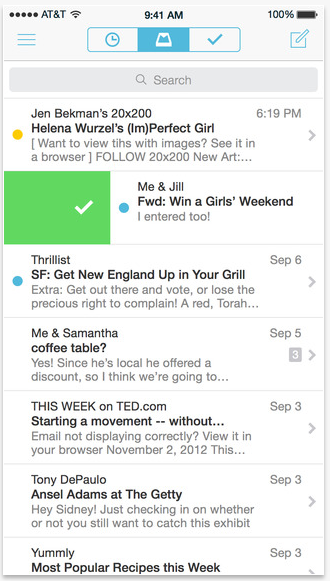
\includegraphics[width=4cm]{media/mailbox1.png}
        \column{.5\textwidth}
            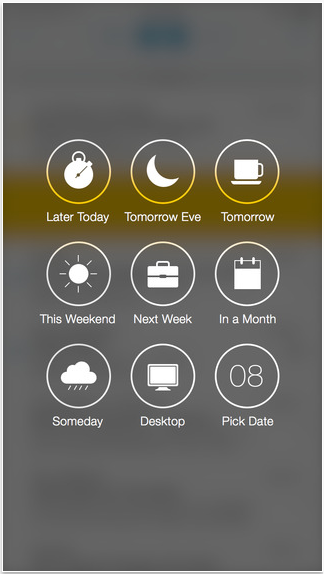
\includegraphics[width=4cm]{media/mailbox2.png}
    \end{columns}
}   

\frame{
    \frametitle{Predicting information usefulness}
    \begin{itemize}
        \item Predicting what users might need to \alert{know} 
        \item Based on past habits, searches, emails, etc.
        \item Based also on human research
        \item Can you be automatically alerted to useful \alert{information}? 
    \end{itemize}
}

\frame{
    \frametitle{Predicting information usefulness: Google Now}
    \begin{itemize}
        \item Baked into Android
    \end{itemize}
    \textbf{Guesses information that might be useful for you, including:}
    \begin{itemize}
        \item Automatic navigation to work/home
        \item Automatic navigation to searched places
        \item Updates on favourite sports teams
        \item Local movie showing times
    \end{itemize}
    \vskip20pt
    \textbf{Presented as}
    \begin{itemize}
        \item `Cards'
        \item Notifications
    \end{itemize}
}

\frame{
    \frametitle{Predicting information usefulness: Google Now}
    \textbf{Guesses information that might be useful for you, including:}
    \begin{itemize}
        \item Automatic navigation to work/home
        \item Automatic navigation to searched places
        \item Updates on favourite sports teams
        \item Local movie showing times
        \item Timezone info (e.g. current time at home)
        \item Weather (where you are, and at home)
    \end{itemize}
    \vskip20pt
    \textbf{Presented as}
    \begin{itemize}
        \item `Cards'
        \item Notifications
    \end{itemize}
}

\frame{
    \frametitle{Predicting information usefulness: Google Now}
    \begin{columns}
        \column{.5\textwidth}
            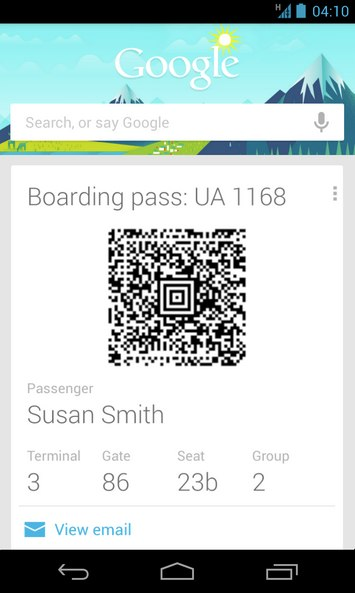
\includegraphics[width=4.5cm]{media/now_boarding.jpg}
        \column{.5\textwidth}
            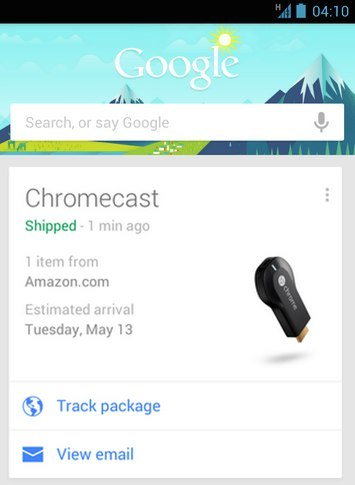
\includegraphics[width=4.5cm]{media/now_shipping.jpg}
    \end{columns}
}

\frame{
    \frametitle{Predicting information usefulness: Google Now}
    \begin{columns}
        \column{.5\textwidth}
            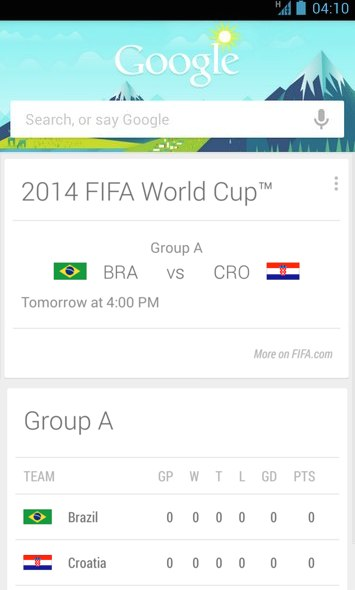
\includegraphics[width=4.5cm]{media/now_sports.jpg}
        \column{.5\textwidth}
            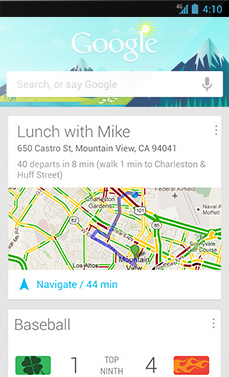
\includegraphics[width=4.5cm]{media/now_navigation.png}
    \end{columns}
}

\frame{
    \frametitle{Predicting information usefulness: Google Now}
    \begin{columns}
        \column{.5\textwidth}
            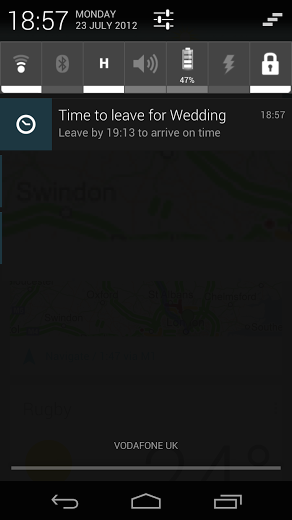
\includegraphics[width=4cm]{media/now_notification1.png}
        \column{.5\textwidth}
            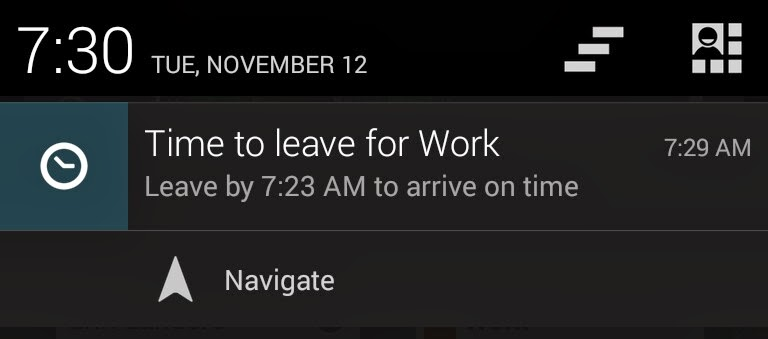
\includegraphics[width=5cm]{media/now_notification2.jpg}
    \end{columns}
}

\frame{
    \frametitle{Predicting behaviour}
    \begin{itemize}
        \item Predicting what users might need to \alert{do}
        \item Based on past habits
        \item Based also on human research        
        \item Can you present the most useful and relevant \alert{actions} to a user?
    \end{itemize}
}

\frame{
    \frametitle{Predicting behaviour: Aviate}
    \begin{columns}
        \column{.8\textwidth}
            \begin{itemize}
                \item Launcher for Android
                \item Updates and rearranges \alert{automatically} depending on
                \begin{itemize}
                    \item Time of day
                    \item Location
                    \item What's happening (e.g. if you're moving)
                    \item Hardware (e.g. if you plug in headphones)
                \end{itemize}
            \end{itemize}
        \column{.2\textwidth}
            
\includegraphics[width=2cm]{media/aviate.png}
    \end{columns}
}

\frame{
    \frametitle{Predicting behaviour: Cover}
    \begin{columns}
        \column{.8\textwidth}
            \begin{itemize}
                \item Lock screen manager for Android 
                \item Updates quick-launch apps depending on
                \begin{itemize}
                    \item Location
                    \item Hardware (e.g. headphones, car)
                \end{itemize}
            \end{itemize}
        \column{.2\textwidth}
            
\includegraphics[width=2cm]{media/cover.png}
    \end{columns}
}

\frame{
    \frametitle{Predicting interruptibility}
    \begin{itemize}
        \item Can systems learn when best to \alert{interrupt} you?
        \item If at a better time, you're more likely to respond appropriately        
        \item Systems can interrupt you with important stuff (phone calls, emails) immediately...
        \item ... and can interrupt you with less imporant stuff (e.g. news stories) at more interruptible times
        \item Various research into interruptibility based on:
        \begin{itemize}
            \item Accelerometer (if you start walking, you may have time to look at your phone)
            \item Time of day (e.g. morning, when alarm is dismissed, etc.)
            \item General learning, depending on user response
        \end{itemize}
    \end{itemize}
}

\frame{
    \frametitle{Predicting interruptibility: ImprompDo}
    \begin{columns}
        \column{.5\textwidth}
            Written by Liam Turner \\ (COMSC 2nd-year PhD student)
            \vskip20pt
            He is researching into human interruptibility
        \column{.5\textwidth}
            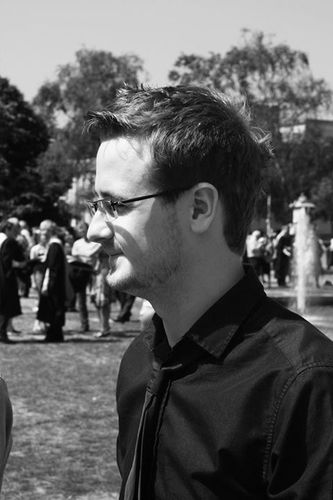
\includegraphics[width=3cm]{media/liam.jpeg}
    \end{columns}     
}

\frame{
    \frametitle{Predicting interruptibility: Imprompdo}
    \begin{columns}
        \column{.8\textwidth}
            \begin{itemize}
                \item Prompts user to check-off items from to-do lists
                \item When prompted:
                \begin{itemize}
                    \item User can ignore (or didn't hear) - auto-dismisses
                    \item User can act (either check item off or not)
                \end{itemize}
                \item Works with 3rd party services: 
                \begin{itemize}
                    \item Google Tasks
                    \item Todoist
                    \item More coming...
                \end{itemize}
                \item Tries to find the best time to prompt user
                \item Available on Google Play if you want to contribute to research in this area!
                \item More info: \alert{cs.cf.ac.uk/imprompdo}
            \end{itemize}
        \column{.2\textwidth}
            
\includegraphics[width=2cm]{media/imprompdo.png}
    \end{columns}
}

\frame{
    \frametitle{Predicting interruptibility: Imprompdo}
    \textbf{Uses several cues:}
    \begin{itemize}
        \item Random
        \item Hourly-based `learner'
        \item After movement (using accelerometer)
        \item `Best time' using machine learning
        \begin{itemize}
            \item Logistic regression on around 12 features
            \item Updates day by day
            \item Works out when you're more likely to respond
        \end{itemize} 
    \end{itemize}
}

\frame{
    \frametitle{Predicting interruptibility: Imprompdo}
    \begin{columns}
        \column{.5\textwidth}
            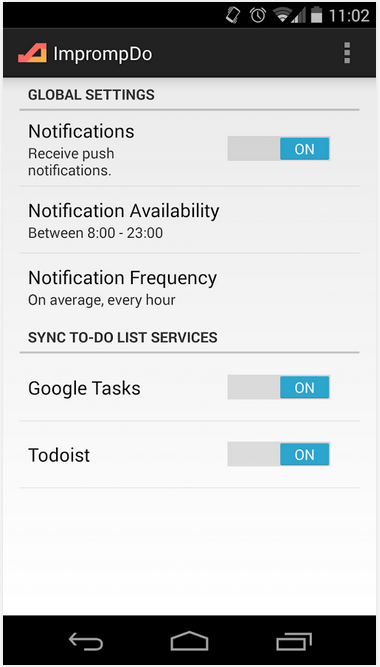
\includegraphics[width=4cm]{media/imprompdo1.png}
        \column{.5\textwidth}
            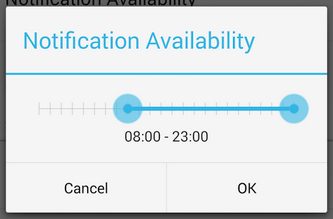
\includegraphics[width=4.5cm]{media/imprompdo2.png}
            \vskip20pt
            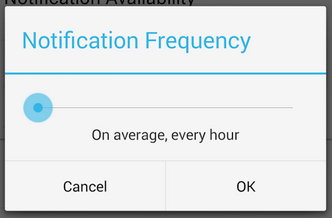
\includegraphics[width=4.5cm]{media/imprompdo3.png}
    \end{columns}
}

\frame{
     \frametitle{Revision questions}
     \begin{enumerate}
        \item How can predictive systems help a user?
        \item In which domain are predictive systems more useful?
        \item How can predictive systems be planned and developed?
        \item What is a push notification? State a disadvantage of push.
        \item How does the Mailbox app help show relevant information?
        \item How does Google Now learn about what to show its users?
        \item What is `interruptibility' in the context of predictive systems?
     \end{enumerate}
}

\frame{
    \frametitle{Summary}
    \begin{itemize}
        \item What predictive systems are
        \item How they can be developed (research, machine learning, etc.)
        \item Push and notifications
        \item Information relevance and Mailbox
        \item Information usefulness and Google Now
        \item Relevant actions, Aviate, and Cover
        \item Interruptibility
    \end{itemize}
}    

\end{document}
